%% Common header for WG21 proposals ? mainly taken from C++ standard draft source
%%

%%--------------------------------------------------
%% basics
%\documentclass[a4paper,11pt,oneside,openany,final,article]{memoir}
\documentclass[a4paper,11pt,oneside,openany,final,article]{memoir}

\usepackage[american]
           {babel}        % needed for iso dates
\usepackage[iso,american]
           {isodate}      % use iso format for dates
\usepackage[final]
           {listings}     % code listings
\usepackage{longtable}    % auto-breaking tables
\usepackage{ltcaption}    % fix captions for long tables
\usepackage{relsize}      % provide relative font size changes
\usepackage{textcomp}     % provide \text{l,r}angle
\usepackage{underscore}   % remove special status of '_' in ordinary text
\usepackage{parskip}      % handle non-indented paragraphs "properly"
\usepackage{array}        % new column definitions for tables
\usepackage[normalem]{ulem}
\usepackage{enumitem}
\usepackage{color}        % define colors for strikeouts and underlines
\usepackage{xcolor}    % needed for blue links

\usepackage{amsmath}      % additional math symbols
\usepackage{mathrsfs}     % mathscr font
\usepackage[final]{microtype}
\usepackage{multicol}
\usepackage{lmodern}
\usepackage[T1]{fontenc}
\usepackage[pdftex, final]{graphicx}
\usepackage[pdftex,
            bookmarks=true,
            bookmarksnumbered=true,
            pdfpagelabels=true,
            pdfpagemode=UseOutlines,
            pdfstartview=FitH,
            linktocpage=true,
            colorlinks=true,
            plainpages=false,
            allcolors={blue}, 
            allbordercolors={white}
           ]{hyperref}
\usepackage{memhfixc}     % fix interactions between hyperref and memoir
\usepackage{url}  % urls in ref.bib
\usepackage{tabularx}  % don't use the C++ standard's fancy tables, they come with captions!

\pdfminorversion=5
\pdfcompresslevel=9
\pdfobjcompresslevel=2

\renewcommand\RSsmallest{5.5pt}  % smallest font size for relsize

%%--------------------------------------------------
%%--------------------------------------------------
%% Layout -- set overall page appearance

%%--------------------------------------------------
%%  set page size, type block size, type block position

\setlrmarginsandblock{2.245cm}{2.245cm}{*}
\setulmarginsandblock{2.5cm}{2.5cm}{*}

%%--------------------------------------------------
%%  set header and footer positions and sizes

\setheadfoot{\onelineskip}{2\onelineskip}
\setheaderspaces{*}{2\onelineskip}{*}

%%--------------------------------------------------
%%  make miscellaneous adjustments, then finish the layout
\setmarginnotes{7pt}{7pt}{0pt}
\checkandfixthelayout

%%--------------------------------------------------
%% If there is insufficient stretchable vertical space on a page,
%% TeX will not properly consider penalties for a good page break,
%% even if \raggedbottom (default) is in effect.
\addtolength{\topskip}{0pt plus 20pt}

%%--------------------------------------------------
%% Paragraph and bullet numbering

\newcounter{Paras}
\counterwithout{section}{chapter}
\setcounter{secnumdepth}{3}

\newcounter{Bullets1}[Paras]
\newcounter{Bullets2}[Bullets1]
\newcounter{Bullets3}[Bullets2]
\newcounter{Bullets4}[Bullets3]

\makeatletter
\newcommand{\parabullnum}[2]{%
\stepcounter{#1}%
\noindent\makebox[0pt][l]{\makebox[#2][r]{%
\scriptsize\raisebox{.7ex}%
{%
\ifnum \value{Paras}>0
\ifnum \value{Bullets1}>0 (\fi%
                          \arabic{Paras}%
\ifnum \value{Bullets1}>0 .\arabic{Bullets1}%
\ifnum \value{Bullets2}>0 .\arabic{Bullets2}%
\ifnum \value{Bullets3}>0 .\arabic{Bullets3}%
\fi\fi\fi%
\ifnum \value{Bullets1}>0 )\fi%
\fi%
}%
\hspace{\@totalleftmargin}\quad%
}}}
\makeatother

\def\pnum{\parabullnum{Paras}{0pt}}

%%--------------------------------------------------
%%--------------------------------------------------
%% Styles
%!TEX root = std.tex
%% styles.tex -- set styles for:
%     chapters
%     pages
%     footnotes

%%--------------------------------------------------
%%  create chapter style

\makechapterstyle{cppstd}{%
  \renewcommand{\beforechapskip}{\onelineskip}
  \renewcommand{\afterchapskip}{\onelineskip}
  \renewcommand{\chapternamenum}{}
  \renewcommand{\chapnamefont}{\chaptitlefont}
  \renewcommand{\chapnumfont}{\chaptitlefont}
  \renewcommand{\printchapternum}{\chapnumfont\thechapter\quad}
  \renewcommand{\afterchapternum}{}
}

%%--------------------------------------------------
%%  create page styles




%%--------------------------------------------------
% set style for main text
\setlength{\parindent}{0pt}
\setlength{\parskip}{1ex}

%%--------------------------------------------------
%% change list item markers to number and em-dash

\renewcommand{\labelitemi}{---\parabullnum{Bullets1}{\labelsep}}
\renewcommand{\labelitemii}{---\parabullnum{Bullets2}{\labelsep}}
\renewcommand{\labelitemiii}{---\parabullnum{Bullets3}{\labelsep}}
\renewcommand{\labelitemiv}{---\parabullnum{Bullets4}{\labelsep}}



%%--------------------------------------------------
%% override some functions from the listings package to avoid bad page breaks
%% (copied verbatim from listings.sty version 1.6 except where commented)
\makeatletter


\def\lst@Init#1{%
    \begingroup
    \ifx\lst@float\relax\else
        \edef\@tempa{\noexpand\lst@beginfloat{lstlisting}[\lst@float]}%
        \expandafter\@tempa
    \fi
    \ifx\lst@multicols\@empty\else
        \edef\lst@next{\noexpand\multicols{\lst@multicols}}
        \expandafter\lst@next
    \fi
    \ifhmode\ifinner \lst@boxtrue \fi\fi
    \lst@ifbox
        \lsthk@BoxUnsafe
        \hbox to\z@\bgroup
             $\if t\lst@boxpos \vtop
        \else \if b\lst@boxpos \vbox
        \else \vcenter \fi\fi
        \bgroup \par\noindent
    \else
        \lst@ifdisplaystyle
            \lst@EveryDisplay
            % make penalty configurable
            \par\lst@beginpenalty
            \vspace\lst@aboveskip
        \fi
    \fi
    \normalbaselines
    \abovecaptionskip\lst@abovecaption\relax
    \belowcaptionskip\lst@belowcaption\relax
    \lst@MakeCaption t%
    \lsthk@PreInit \lsthk@Init
    \lst@ifdisplaystyle
        \global\let\lst@ltxlabel\@empty
        \if@inlabel
            \lst@ifresetmargins
                \leavevmode
            \else
                \xdef\lst@ltxlabel{\the\everypar}%
                \lst@AddTo\lst@ltxlabel{%
                    \global\let\lst@ltxlabel\@empty
                    \everypar{\lsthk@EveryLine\lsthk@EveryPar}}%
            \fi
        \fi
        % A section heading might have set \everypar to apply a \clubpenalty
        % to the following paragraph, changing \everypar in the process.
        % Unconditionally overriding \everypar is a bad idea.
        % \everypar\expandafter{\lst@ltxlabel
        %                      \lsthk@EveryLine\lsthk@EveryPar}%
    \else
        \everypar{}\let\lst@NewLine\@empty
    \fi
    \lsthk@InitVars \lsthk@InitVarsBOL
    \lst@Let{13}\lst@MProcessListing
    \let\lst@Backslash#1%
    \lst@EnterMode{\lst@Pmode}{\lst@SelectCharTable}%
    \lst@InitFinalize}

\def\lst@DeInit{%
    \lst@XPrintToken \lst@EOLUpdate
    \global\advance\lst@newlines\m@ne
    \lst@ifshowlines
        \lst@DoNewLines
    \else
        \setbox\@tempboxa\vbox{\lst@DoNewLines}%
    \fi
    \lst@ifdisplaystyle \par\removelastskip \fi
    \lsthk@ExitVars\everypar{}\lsthk@DeInit\normalbaselines\normalcolor
    \lst@MakeCaption b%
    \lst@ifbox
        \egroup $\hss \egroup
        \vrule\@width\lst@maxwidth\@height\z@\@depth\z@
    \else
        \lst@ifdisplaystyle
            % make penalty configurable
            \par\lst@endpenalty
            \vspace\lst@belowskip
        \fi
    \fi
    \ifx\lst@multicols\@empty\else
        \def\lst@next{\global\let\@checkend\@gobble
                      \endmulticols
                      \global\let\@checkend\lst@@checkend}
        \expandafter\lst@next
    \fi
    \ifx\lst@float\relax\else
        \expandafter\lst@endfloat
    \fi
    \endgroup}


\def\lst@NewLine{%
    \ifx\lst@OutputBox\@gobble\else
        \par
        % add configurable penalties
        \lst@ifeolsemicolon
          \lst@semicolonpenalty
          \lst@eolsemicolonfalse
        \else
          \lst@domidpenalty
        \fi
        % Manually apply EveryLine and EveryPar; do not depend on \everypar
        \noindent \hbox{}\lsthk@EveryLine%
        % \lsthk@EveryPar uses \refstepcounter which balloons the PDF
    \fi
    \global\advance\lst@newlines\m@ne
    \lst@newlinetrue}

% new macro for empty lines, avoiding an \hbox that cannot be discarded
\def\lst@DoEmptyLine{%
  \ifvmode\else\par\fi\lst@emptylinepenalty
  \vskip\parskip
  \vskip\baselineskip
  % \lsthk@EveryLine has \lst@parshape, i.e. \parshape, which causes an \hbox
  % \lsthk@EveryPar increments line counters; \refstepcounter balloons the PDF
  \global\advance\lst@newlines\m@ne
  \lst@newlinetrue}

\def\lst@DoNewLines{
    \@whilenum\lst@newlines>\lst@maxempty \do
        {\lst@ifpreservenumber
            \lsthk@OnEmptyLine
            \global\advance\c@lstnumber\lst@advancelstnum
         \fi
         \global\advance\lst@newlines\m@ne}%
    \@whilenum \lst@newlines>\@ne \do
        % special-case empty printing of lines
        {\lsthk@OnEmptyLine\lst@DoEmptyLine}%
    \ifnum\lst@newlines>\z@ \lst@NewLine \fi}

% add keys for configuring before/end vertical penalties
\lst@Key{beginpenalty}\relax{\def\lst@beginpenalty{\penalty #1}}
\let\lst@beginpenalty\@empty
\lst@Key{midpenalty}\relax{\def\lst@midpenalty{\penalty #1}}
\let\lst@midpenalty\@empty
\lst@Key{endpenalty}\relax{\def\lst@endpenalty{\penalty #1}}
\let\lst@endpenalty\@empty
\lst@Key{emptylinepenalty}\relax{\def\lst@emptylinepenalty{\penalty #1}}
\let\lst@emptylinepenalty\@empty
\lst@Key{semicolonpenalty}\relax{\def\lst@semicolonpenalty{\penalty #1}}
\let\lst@semicolonpenalty\@empty

\lst@AddToHook{InitVars}{\let\lst@domidpenalty\@empty}
\lst@AddToHook{InitVarsEOL}{\let\lst@domidpenalty\lst@midpenalty}

% handle semicolons and closing braces (could be in \lstdefinelanguage as well)
\def\lst@eolsemicolontrue{\global\let\lst@ifeolsemicolon\iftrue}
\def\lst@eolsemicolonfalse{\global\let\lst@ifeolsemicolon\iffalse}
\lst@AddToHook{InitVars}{
  \global\let\lst@eolsemicolonpending\@empty
  \lst@eolsemicolonfalse
}
% If we found a semicolon or closing brace while parsing the current line,
% inform the subsequent \lst@NewLine about it for penalties.
\lst@AddToHook{InitVarsEOL}{%
  \ifx\lst@eolsemicolonpending\relax
    \lst@eolsemicolontrue
    \global\let\lst@eolsemicolonpending\@empty
  \fi%
}
\lst@AddToHook{SelectCharTable}{%
  % In theory, we should only detect trailing semicolons or braces,
  % but that would require un-doing the marking for any other character.
  % The next best thing is to undo the marking for closing parentheses,
  % because loops or if statements are the only places where we will
  % reasonably have a semicolon in the middle of a line, and those all
  % end with a closing parenthesis.
  \lst@DefSaveDef{41}\lstsaved@closeparen{%    handle closing parenthesis
    \lstsaved@closeparen
    \ifnum\lst@mode=\lst@Pmode    % regular processing mode (not a comment)
      \global\let\lst@eolsemicolonpending\@empty  % undo semicolon setting
    \fi%
  }%
  \lst@DefSaveDef{59}\lstsaved@semicolon{%     handle semicolon
    \lstsaved@semicolon
    \ifnum\lst@mode=\lst@Pmode    % regular processing mode (not a comment)
      \global\let\lst@eolsemicolonpending\relax
    \fi%
  }%
  \lst@DefSaveDef{125}\lstsaved@closebrace{%   handle closing brace
    \lst@eolsemicolonfalse        % do not break before a closing brace
    \lstsaved@closebrace          % might invoke \lst@NewLine
    \ifnum\lst@mode=\lst@Pmode    % regular processing mode (not a comment)
      \global\let\lst@eolsemicolonpending\relax
    \fi%
  }%
}

\makeatother


%%--------------------------------------------------
%%--------------------------------------------------
%% Macros
%!TEX root = std.tex
% Definitions and redefinitions of special commands

%%--------------------------------------------------
%% Difference markups
\definecolor{addclr}{rgb}{0,0.4,0.05}
\definecolor{remclr}{rgb}{1,0,0}
\definecolor{noteclr}{rgb}{0,0,1}

\renewcommand{\added}[1]{\textcolor{addclr}{\uline{#1}}}
\newcommand{\removed}[1]{\textcolor{remclr}{\sout{#1}}}
\renewcommand{\changed}[2]{\removed{#1}\added{#2}}

\newcommand{\nbc}[1]{[#1]\ }
\newcommand{\addednb}[2]{\added{\nbc{#1}#2}}
\newcommand{\removednb}[2]{\removed{\nbc{#1}#2}}
\newcommand{\changednb}[3]{\removednb{#1}{#2}\added{#3}}
\newcommand{\remitem}[1]{\item\removed{#1}}

\newcommand{\ednote}[1]{\textcolor{noteclr}{[Editor's note: #1] }}
% \newcommand{\ednote}[1]{}

\newenvironment{addedblock}
{
\color{addclr}
}
{
\color{black}
}
\newenvironment{removedblock}
{
\color{remclr}
}
{
\color{black}
}

%%--------------------------------------------------
% General code style
\newcommand{\CodeStyle}{\ttfamily}
\newcommand{\CodeStylex}[1]{\texttt{#1}}
\newcommand{\CodeStylexul}[1]{\underline{\texttt{#1}}}

% Code and definitions embedded in text.
\newcommand{\tcode}[1]{\CodeStylex{#1}}
\newcommand{\tcodeul}[1]{\CodeStylexul{#1}}
\newcommand{\techterm}[1]{\textit{#1}}
\newcommand{\defnx}[2]{\indexdefn{#2}\textit{#1}}
\newcommand{\defn}[1]{\defnx{#1}{#1}}
\newcommand{\term}[1]{\textit{#1}}
\newcommand{\grammarterm}[1]{\textit{#1}}
\newcommand{\grammartermnc}[1]{\textit{#1}\nocorr}
\newcommand{\placeholder}[1]{\textit{#1}}
\newcommand{\placeholdernc}[1]{\textit{#1\nocorr}}

%%--------------------------------------------------
%% allow line break if needed for justification
\newcommand{\brk}{\discretionary{}{}{}}

%%--------------------------------------------------
%% Macros for funky text
\newcommand{\Cpp}{\texorpdfstring{C\kern-0.05em\protect\raisebox{.35ex}{\textsmaller[2]{+\kern-0.05em+}}}{C++}}
\newcommand{\CppIII}{\Cpp{} 2003}
\newcommand{\CppXI}{\Cpp{} 2011}
\newcommand{\CppXIV}{\Cpp{} 2014}
\newcommand{\CppXVII}{\Cpp{} 2017}
\newcommand{\opt}[1]{\ifthenelse{\equal{#1}{}}
    {\PackageError{main}{argument must not be empty}{}}
    {#1\ensuremath{_\mathit{opt}}}}
\newcommand{\dcr}{-{-}}
\newcommand{\bigoh}[1]{\ensuremath{\mathscr{O}(#1)}}

% Make all tildes a little larger to avoid visual similarity with hyphens.
\renewcommand{\~}{\textasciitilde}
\let\OldTextAsciiTilde\textasciitilde
\renewcommand{\textasciitilde}{\protect\raisebox{-0.17ex}{\larger\OldTextAsciiTilde}}
\newcommand{\caret}{\char`\^}

%%--------------------------------------------------
%% States and operators
\newcommand{\state}[2]{\tcode{#1}\ensuremath{_{#2}}}
\newcommand{\bitand}{\ensuremath{\, \mathsf{bitand} \,}}
\newcommand{\bitor}{\ensuremath{\, \mathsf{bitor} \,}}
\newcommand{\xor}{\ensuremath{\, \mathsf{xor} \,}}
\newcommand{\rightshift}{\ensuremath{\, \mathsf{rshift} \,}}
\newcommand{\leftshift}[1]{\ensuremath{\, \mathsf{lshift}_#1 \,}}

%% Notes and examples
\newcommand{\noteintro}[1]{[\,\textit{#1:}\space}
\newcommand{\noteoutro}[1]{\textit{\,---\,end #1}\,]}
\newenvironment{note}[1][Note]{\noteintro{#1}}{\noteoutro{note}\space}
\newenvironment{example}[1][Example]{\noteintro{#1}}{\noteoutro{example}\space}

%% Library function descriptions
\newcommand{\Fundescx}[1]{\textit{#1}}
\newcommand{\Fundesc}[1]{\Fundescx{#1:}\space}
\newcommand{\required}{\Fundesc{Required behavior}}
\newcommand{\requires}{\Fundesc{Requires}}
\newcommand{\effects}{\Fundesc{Effects}}
\newcommand{\postconditions}{\Fundesc{Postconditions}}
\newcommand{\returns}{\Fundesc{Returns}}
\newcommand{\throws}{\Fundesc{Throws}}
\newcommand{\default}{\Fundesc{Default behavior}}
\newcommand{\complexity}{\Fundesc{Complexity}}
\newcommand{\remarks}{\Fundesc{Remarks}}
\newcommand{\errors}{\Fundesc{Error conditions}}
\newcommand{\sync}{\Fundesc{Synchronization}}
\newcommand{\implimits}{\Fundesc{Implementation limits}}
\newcommand{\replaceable}{\Fundesc{Replaceable}}
\newcommand{\returntype}{\Fundesc{Return type}}
\newcommand{\cvalue}{\Fundesc{Value}}
\newcommand{\ctype}{\Fundesc{Type}}
\newcommand{\ctypes}{\Fundesc{Types}}
\newcommand{\dtype}{\Fundesc{Default type}}
\newcommand{\ctemplate}{\Fundesc{Class template}}
\newcommand{\templalias}{\Fundesc{Alias template}}

%% Cross reference
\newcommand{\xref}{\textsc{See also:}\space}

%% Inline parenthesized reference
\newcommand{\iref}[1]{\nolinebreak[3] (\ref{#1})}

%% NTBS, etc.
\newcommand{\NTS}[1]{\textsc{#1}}
\newcommand{\ntbs}{\NTS{ntbs}}
\newcommand{\ntmbs}{\NTS{ntmbs}}
% The following are currently unused:
% \newcommand{\ntwcs}{\NTS{ntwcs}}
% \newcommand{\ntcxvis}{\NTS{ntc16s}}
% \newcommand{\ntcxxxiis}{\NTS{ntc32s}}

%% Code annotations
\newcommand{\EXPO}[1]{\textit{#1}}
\newcommand{\expos}{\EXPO{exposition only}}
\newcommand{\impdef}{\EXPO{implementation-defined}}
\newcommand{\impdefnc}{\EXPO{implementation-defined\nocorr}}
\newcommand{\impdefx}[1]{\indeximpldef{#1}\EXPO{implementation-defined}}
\newcommand{\notdef}{\EXPO{not defined}}

\newcommand{\UNSP}[1]{\textit{\texttt{#1}}}
\newcommand{\UNSPnc}[1]{\textit{\texttt{#1}\nocorr}}
\newcommand{\unspec}{\UNSP{unspecified}}
\newcommand{\unspecnc}{\UNSPnc{unspecified}}
\newcommand{\unspecbool}{\UNSP{unspecified-bool-type}}
\newcommand{\seebelow}{\UNSP{see below}}
\newcommand{\seebelownc}{\UNSPnc{see below}}
\newcommand{\unspecuniqtype}{\UNSP{unspecified unique type}}
\newcommand{\unspecalloctype}{\UNSP{unspecified allocator type}}

\newcommand{\EXPLICIT}{\textit{\texttt{EXPLICIT}\nocorr}}

%% Manual insertion of italic corrections, for aligning in the presence
%% of the above annotations.
\newlength{\itcorrwidth}
\newlength{\itletterwidth}
\newcommand{\itcorr}[1][]{%
 \settowidth{\itcorrwidth}{\textit{x\/}}%
 \settowidth{\itletterwidth}{\textit{x\nocorr}}%
 \addtolength{\itcorrwidth}{-1\itletterwidth}%
 \makebox[#1\itcorrwidth]{}%
}

%% Double underscore
\newcommand{\ungap}{\kern.5pt}
\newcommand{\unun}{\textunderscore\ungap\textunderscore}
\newcommand{\xname}[1]{\tcode{\unun\ungap#1}}
\newcommand{\mname}[1]{\tcode{\unun\ungap#1\ungap\unun}}

%% An elided code fragment, /* ... */, that is formatted as code.
%% (By default, listings typeset comments as body text.)
%% Produces 9 output characters.
\newcommand{\commentellip}{\tcode{/* ...\ */}}

%% Ranges
\newcommand{\Range}[4]{\tcode{#1#3,\penalty2000{} #4#2}}
\newcommand{\crange}[2]{\Range{[}{]}{#1}{#2}}
\newcommand{\brange}[2]{\Range{(}{]}{#1}{#2}}
\newcommand{\orange}[2]{\Range{(}{)}{#1}{#2}}
\newcommand{\range}[2]{\Range{[}{)}{#1}{#2}}

%% Change descriptions
\newcommand{\diffdef}[1]{\hfill\break\textbf{#1:}\space}
\newcommand{\diffref}[1]{\pnum\textbf{Affected subclause:} \ref{#1}}
\newcommand{\change}{\diffdef{Change}}
\newcommand{\rationale}{\diffdef{Rationale}}
\newcommand{\effect}{\diffdef{Effect on original feature}}
\newcommand{\difficulty}{\diffdef{Difficulty of converting}}
\newcommand{\howwide}{\diffdef{How widely used}}

%% Miscellaneous
\newcommand{\uniquens}{\placeholdernc{unique}}
\newcommand{\stage}[1]{\item[Stage #1:]}
\newcommand{\doccite}[1]{\textit{#1}}
\newcommand{\cvqual}[1]{\textit{#1}}
\newcommand{\cv}{\cvqual{cv}}
\newcommand{\numconst}[1]{\textsl{#1}}
\newcommand{\logop}[1]{{\footnotesize #1}}

%%--------------------------------------------------
%% Environments for code listings.

% We use the 'listings' package, with some small customizations.  The
% most interesting customization: all TeX commands are available
% within comments.  Comments are set in italics, keywords and strings
% don't get special treatment.

\lstset{language=C++,
        basicstyle=\small\CodeStyle,
        keywordstyle=,
        stringstyle=,
        xleftmargin=1em,
        showstringspaces=false,
        commentstyle=\itshape\rmfamily,
        columns=fullflexible,
        keepspaces=true,
        texcl=true}


% Our usual abbreviation for 'listings'.  Comments are in
% italics.  Arbitrary TeX commands can be used if they're
% surrounded by @ signs.
\newcommand{\CodeBlockSetup}{
 \lstset{escapechar=@, aboveskip=\parskip, belowskip=0pt,
         midpenalty=500, endpenalty=-50,
         emptylinepenalty=-250, semicolonpenalty=0,rulecolor=\color{black}}
 \renewcommand{\tcode}[1]{\textup{\CodeStylex{##1}}}
 \newcommand{\textbfx}[1]{\textup{\CodeStylex{\color{blue}\textbf{##1}}}}
 \renewcommand{\techterm}[1]{\textit{\CodeStylex{##1}}}
 \renewcommand{\term}[1]{\textit{##1}}
 \renewcommand{\grammarterm}[1]{\textit{##1}}
}

\lstnewenvironment{codeblock}{\CodeBlockSetup}{}



\newcommand{\CodeBlockAddSetup}{
 \lstset{basicstyle=\small\CodeStyle\color{addclr},escapechar=@, aboveskip=\parskip, belowskip=0pt,
         midpenalty=500, endpenalty=-50,
         emptylinepenalty=-250, semicolonpenalty=0}
 \renewcommand{\tcode}[1]{\textup{\CodeStylex{##1}}}
 \renewcommand{\techterm}[1]{\textit{\CodeStylex{##1}}}
 \renewcommand{\term}[1]{\textit{##1}}
 \renewcommand{\grammarterm}[1]{\textit{##1}}
}

\lstnewenvironment{codeblockAdd}{\CodeBlockAddSetup}{}




% Our usual abbreviation for 'listings'.  Comments are in
% italics.  Arbitrary TeX commands can be used if they're
% surrounded by @ signs.
\newcommand{\CodeBlockSetupSmall}{
 \tiny
 \lstset{escapechar=@, aboveskip=\parskip, belowskip=0pt,
         midpenalty=500, endpenalty=-50, basicstyle=\small,
         emptylinepenalty=-250, semicolonpenalty=0}
 \renewcommand{\tcode}[1]{\textup{\CodeStylex{##1}}}
 \renewcommand{\techterm}[1]{\textit{\CodeStylex{##1}}}
 \renewcommand{\term}[1]{\textit{##1}}
 \renewcommand{\grammarterm}[1]{\textit{##1}}
}

\lstnewenvironment{codeblocksmall}{\CodeBlockSetupSmall}{}



% An environment for command / program output that is not C++ code.
\lstnewenvironment{outputblock}{\lstset{language=}}{}

% A code block in which single-quotes are digit separators
% rather than character literals.
\lstnewenvironment{codeblockdigitsep}{
 \CodeBlockSetup
 \lstset{deletestring=[b]{'}}
}{}

% Permit use of '@' inside codeblock blocks (don't ask)
\makeatletter
\newcommand{\atsign}{@}
\makeatother

%%--------------------------------------------------
%% Indented text
\newenvironment{indented}[1][]
{\begin{indenthelper}[#1]\item\relax}
{\end{indenthelper}}

%%--------------------------------------------------
%% Library item descriptions
\lstnewenvironment{itemdecl}
{
 \lstset{escapechar=@,
 xleftmargin=0em,
 midpenalty=500,
 semicolonpenalty=-50,
 endpenalty=3000,
 aboveskip=2ex,
 belowskip=0ex	% leave this alone: it keeps these things out of the
				% footnote area
 }
}
{
}

\newenvironment{itemdescr}
{
 \begin{indented}[beginpenalty=3000, endpenalty=-300]}
{
 \end{indented}
}

%%--------------------------------------------------
%% add special hyphenation rules
\hyphenation{tem-plate ex-am-ple in-put-it-er-a-tor name-space name-spaces non-zero}

%%--------------------------------------------------
%% turn off all ligatures inside \texttt
\DisableLigatures{encoding = T1, family = tt*}



%%%%%%%%%%%%%%%%%%%% lundberg, normal-sized footnote text (we are not all young...)
\renewcommand{\footnotesize}{\normalsize}

%%%%%%%%%%%%%%%%%%%%%%%%%%%%%%%%%%
\newcommand{\dblquotes}[1]{``#1''}







%\addtolength{\textheight}{7em}
\let\oldaddcontentsline\addcontentsline% Store \addcontentsline

\sloppy
\setcounter{tocdepth}{5}
%%%%%%%%%%%%%%%%%%%%%%%%%%%%%%%%%%%%%%%%
%\usepackage{showframe}
\usepackage{lipsum}
\usepackage{xcolor}

\usepackage{enumitem}
\newlist{myQuoteEnumerate}{enumerate}{2}% Set max nesting depth
\setlist[myQuoteEnumerate,1]{label=(\arabic*)}% Use numbers for level 1
\setlist[myQuoteEnumerate,2]{label=(\alph*)}%   Use letters for level 2

\newenvironment{MyQuote}{%
    \begin{myQuoteEnumerate}[resume=*,series=MyQuoteSeries]%
    \color{blue}%
    \item \begin{quote}%
}{%
    \end{quote}%
    \end{myQuoteEnumerate}%
}%
%%%%%%%%%%%%%%%%%%%%%%%%%%
\usepackage{lineno}
%\iffalse
\usepackage{xcolor}
\usepackage{lineno}
\usepackage{lipsum}
\makeatletter
\renewcommand{\linenumberfont}{\fontsize{12pt}{3pt}\normalfont\smaller\color{gray}}
\makeatother
%\usepackage{lineno}
%\linenumbers
%\fi
%%%%%%%%%%%%%%%%%%%%%%%%
\linespread{1.0}
%%%%%%%%%%%%%%%%%%%%%%%%
\makeatletter
\renewcommand\tableofcontents{%
    \@starttoc{toc}%
}
\makeatother


\begin{document}
\vspace*{-4em}
\title{\tcode{Generalisation of nth_element to a range of nths}}
\author{
Johan Lundberg\\
}
\date{} %unused. Type date explicitly below.
\maketitle
\vspace*{-3em}

\begin{tabular}{ll}
Document \#:& D2375R1\\
Date: &2022-01-02 \\
Project: & Programming Language C++ \\
Audience: & LEWG \\
Email: &\href{mailto:lundberj@gmail.com}{lundberj@gmail.com}
\end{tabular}

\iffalse %%% FOR ONLINE ABSTRACT
The paper proposes a generalisation of \tcode{std::nth_element}, taking a sorted range of iterators instead of a single nth element iterator, allowing arbitrary partial sorting of any sortable range.
The use and analysis of such algorithms is widespread and mature\cite{Alsuwaiyel2001,Kaligosi2006,Panh2002,lent1996,Shen1997} and is available to Python programmers as numpy.partition\cite{NpPart,NPImpl} since 2014.
\fi

\subsection*{Contents}
\renewcommand{\baselinestretch}{1.0}\normalsize
\tableofcontents
\renewcommand{\baselinestretch}{1.2}\normalsize

\newpage\subsection*{Revision history vs R0}
\addcontentsline{toc}{section}{Revision history}

2021-12-16: Added clarifications and more background, explanations, wording clarifications, references, summarized performance study, applications, more questions/answers. --Based on feedback and material sent to SG9 list 2021-12-09. Added images for equalization example. Added example of \emph{Before} with projections and more examples. -- 
2021-12-26: Added explanatory images to the introduction. --  
2021-12-28: Rebased wording and synopsis to C++23 draft. 2021-01-02: Updated to new performance result. Clarified that complexity is expected. Misc polishing. 

\section{Introduction}
The paper proposes a generalisation of \tcode{std::nth_element}, taking a sorted range of iterators instead of a single \tcode{nth} iterator, allowing arbitrary partial sorting of any sortable range.

The use and analysis of such algorithms is widespread and mature\cite{Alsuwaiyel2001,Panh2002,lent1996,Shen1997} under the name \emph{multiple selection} or \emph{multiselect}. It is available to Python programmers as \tcode{numpy.partition}\cite{NpPart,NPImpl} since 2014. 

The single-nth \tcode{nth_element} algorithm has been part of the C++ standard library since the beginning\cite{StepLee95}, introduced as \dblquotes{\ldots  the  element  in  the  position  pointed  to  by nth  is  the  element  that  would  be  in  that position if the whole range were sorted. Also for any iterator i in the range [first, nth) and any iterator j in the range [nth, last) it holds that !(*i > *j) or comp(*i, *j) == false. It is linear on the average.}

\emph{This} proposal extends the usability of \tcode{std::nth_element} to multiple \tcode{nths}. 
That is, the previously stated post condition holds for all nth in \tcode{nths}. In other words, at each nth the range is arranged as if sorted, and all elements after each nth are no less than the element at that location. 

Just as with the current standard single-nth version of \tcode{std::nth_element} the purpose is \emph{faster operation}, but just as with the single-nth version, there is additional \emph{semantic clarity} in performing only the required partitioning. 
In this specific sense it's in the same category as \tcode{std::partial_sort}.

Possible implementations of the range-of-nths algorithm is provided (section \ref{Implementation}, and \cite{p2375RefImpl}).
It translates naturally to \tcode{std::ranges} versions.

Current alternatives are either at least somewhat hard to write correctly and/or less performant.

To clarify what is new, the addition is here called \tcode{std::multi_nth_element}, but the proposed wording overloads \tcode{std::nth_element}. 

\newpage
\subsection{Visual explanation}

As example data, consider the permuted integers [100,126) at index [0,26) and the sorted counterpart:

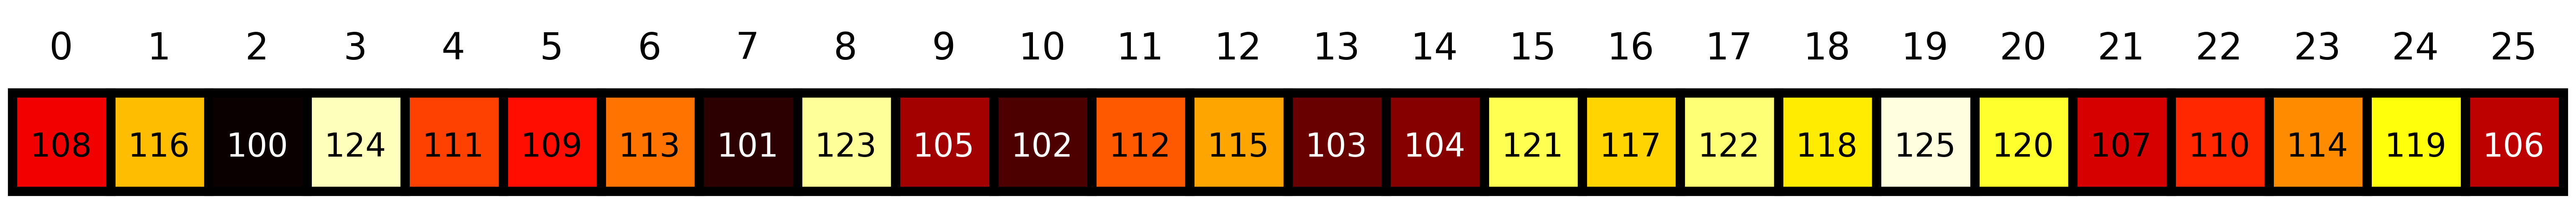
\includegraphics[width=0.999\textwidth]{plotting/figs/rnd.png}

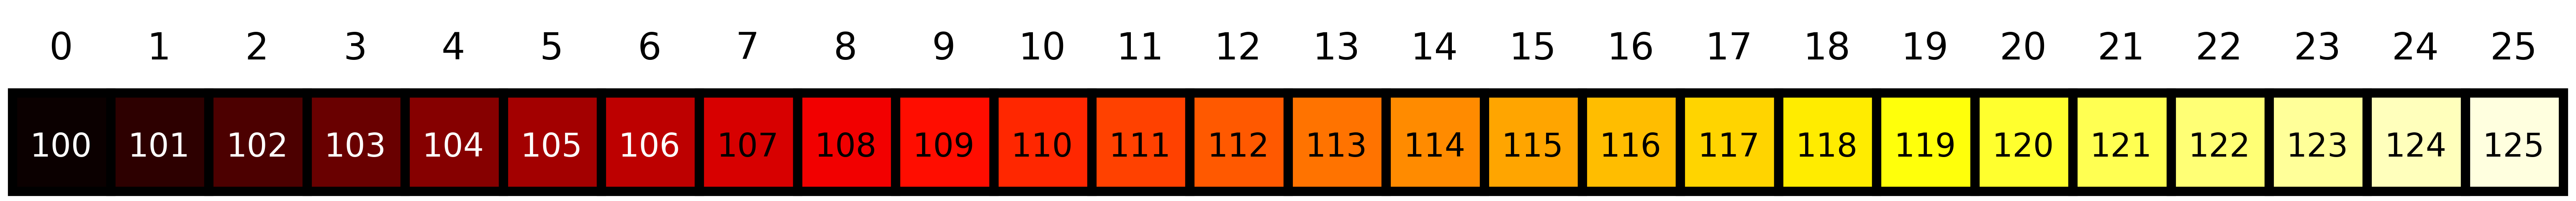
\includegraphics[width=0.999\textwidth]{plotting/figs/sort.png}

\subsubsection*{Single-nth \tcode{nth_element}}

What the current-standard \tcode{std::nth_element} does is to rearrange the data in relation to a specified nth position, as described in the previous section. With our concrete example, with {nth = begin+7}, the effect is that the element at nth is the element (in our case: 107) that  would  be  in  that position if the whole range were sorted, and all subsequent values are no less than that value:

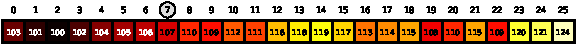
\includegraphics[width=0.999\textwidth]{plotting/figs/1a.pdf},

or for \tcode{nth = begin+20}:

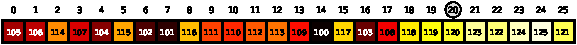
\includegraphics[width=0.999\textwidth]{plotting/figs/1b.pdf}.

\subsubsection*{Multi-nth \tcode{nth_element}}

This proposal adds support for multiple selection. That is, the possibility to provide a range of nths, such as \tcode{\{begin+7, begin+20\}} :

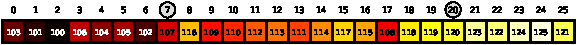
\includegraphics[width=0.999\textwidth]{plotting/figs/2.pdf}

or at \tcode{\{begin+7, begin+12, begin+20\}}:

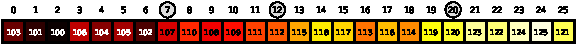
\includegraphics[width=0.999\textwidth]{plotting/figs/3.pdf}

or  at \tcode{\{begin+5, begin+6, begin+14, begin+15\}}:

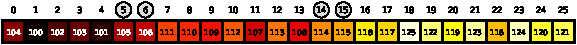
\includegraphics[width=0.999\textwidth]{plotting/figs/qs.pdf}

\newpage
\section{The algorithm}
\label{Implementation}
\label{Implement}

Several implementations are provided\cite{p2375RefImpl}. The first is \tcode{multi_quick_select}, which can either be described as the natural extension of quick select, or as a shallow quick sort. The second implementation, here called \tcode{bisect_nths}\footnote{Analyzed in \cite{Alsuwaiyel2001}, in context of 
parallel versions. Builds on refs \cite{Akl1984,Akl1989,Shen1997}.} 
 is in a sense simpler, and is shown below. It works by bisecting \tcode{nths}, partitions the data using the single-nth \tcode{nth_element}, and recurses. 

\begin{codeblock}
// multi_nth_element implemented using bisect_nths
template< class RandomAccessIterator, class RandomAccessIteratorNths >
constexpr void @\textbfx{multi_nth_element}@(RandomAccessIterator first, 
  RandomAccessIteratorNths nth_first, RandomAccessIteratorNths nth_last, 
  RandomAccessIterator last){
  if (last - first <= 32) { @\textbfx{std::sort(first, last)}@; return; }
  const auto nth_dist = nth_last - nth_first;
  if (nth_dist == 0 || *nth_first == last) return;
  const auto nth_mid = nth_first + nth_dist / 2;
  const auto at_nth_mid = *nth_mid;
  @\textbfx{nth_element(first, at_nth_mid, last)}@;
  @\textbfx{multi_nth_element(first, nth_first, nth_mid, at_nth_mid)}@;
  if (at_nth_mid != last){
    const auto nth_left = std::upper_bound(nth_mid, nth_last, at_nth_mid );
    @\textbfx{multi_nth_element(at_nth_mid + 1, nth_left, nth_last, last)}@;
  }
}
\end{codeblock}


The complexity for both \tcode{multi_quick_select} and \tcode{bisect_nths} is \mbox{O(N log m)} on average, where \mbox{N = last - first} and m is the number of unique elements in nths. To be compared with \mbox{O(N)} on average for current \tcode{std::nth_element}. 

In many applications m is constant and the complexity as function of N alone is naturally linear on average. On the other hand, in the worst case m varies with N as \mbox{m = N}, and the whole container is sorted. For parallel versions (overloads taking an ExecutionPolicy) it is reasonable to leave freedom to implementers to do a full parallel sort and allow \mbox{O(N log N)}.

Python has numpy.partition\cite{NpPart} as their incarnation of \tcode{ntn_element}. 
It also support multi selection, and the implementation\cite{NPImpl}(in C++) uses \mbox{Introselect\cite{Musser1997}} by specification%
\footnote{Interestingly, Musser only hints on single element selection as a future extension of introsort. 
Further: numpy.partition do not state complexity in terms of M (the size of nths) or m (the number of unique nths), 
but promises \emph{worst case} O(N). It appears to be \mbox{$\sim$ N log M} for reasonable M, 
to become \mbox{$\sim$ N $\cdot$ M} for large M, such as M>1e4, N=1e6. }.

Further references on the subject are \cite{Kaligosi2006,Panh2002}.

\newpage
\section{Tony Tables (Before/After)}

Existing alternatives are to sort the whole container or to figure out a series of calls to e.g. \tcode{nth_element} and \tcode{partial_sort}. 
The examples below could be the linear time partitioning of messages to be
processed into fixed sized priority buckets, keeping or dropping remaining messages. Or finding the fastest 25, 100, and 1000 race participants in linear time. 
The partitions themselves form half open ranges so it's easy to e.g. sort and
print the 100th up to the 1000th fastest runners by name. 

Context: partitioning into a fixed number of slots
\begin{codeblock}
vector<decltype(v)::iterator> nths;
for(size_t slot=1; slot<16 ; ++slot){
	nths.push_back(v.begin()+ min(slot*2048,N));
}
\end{codeblock}
or at some other arbitrary iterators in the inclusive range [first,last].
\begin{codeblock}
auto nths=vector{v.begin()+25,v.begin()+100,v.begin()+1000}; 
\end{codeblock}

\subsection*{After \textnormal{ Simple and O(N)}}

For all examples, the Tony Tables--\emph{After} case is the same:\newline

\hspace{3ex}\begin{tabular}{|l|} 
  \hline 
  \textbf{$\star \star$ After $\star \star$} \\
  \hline 
\begin{codeblock} 
multi_nth_element(v, nths, pred);
\end{codeblock}\\[1em]
or, for the examples using a projection:
\\
\begin{codeblock} 
multi_nth_element(v, nths, pred, proj);
\end{codeblock} 
\\
\hline 
\end{tabular} 


\subsection*{Alternative 1a: Hand-wired bisection for nths of known size 3. O(N) but messy}

\hspace{3ex}\begin{tabular}{|l|} 
  \hline 
  \textbf{Before} \\
  \hline 
\begin{codeblock} 
nth_element(v.begin(), nths[1], v.end(), pred);
nth_element(v.begin(), nths[0], nths[1], pred);
nth_element(nths[1]+1, nths[2], v.end(), pred);
\end{codeblock} 
\\
\hline 
\end{tabular} 

Did we get this right? Is it correct for repeated nths or empty v?
This is an attempt at manually figuring out and hand-inlining \emph{this} proposal for a know nths size equal to 3.

If we are using a projection, we must use sub-ranges or something to the same effect (and with the same risk of corner-case bugs, eg missed +1 at the right places):

\hspace{3ex}\begin{tabular}{|l|} 
  \hline 
  \textbf{Before} \\
  \hline 
\begin{codeblock} 
ranges::nth_element(v, nths[1], pred, proj);
ranges::nth_element(sub_range(v.begin(),nths[1]), nths[0], pred, proj);
ranges::nth_element(sub_range(nths[1]+1,v.end()), nths[2], pred, proj);
\end{codeblock} 
\\
\hline 
\end{tabular} 
\subsection*{Alternative 1b: Hand-wired bisection for nths of known size 5. O(N) but messy}

\hspace{3ex}\begin{tabular}{|l|} 
  \hline 
  \textbf{Before} \\
  \hline 
\begin{codeblock} 
nth_element(v.begin(), nths[5/2-1], v.end(), pred);
nth_element(v.begin(), nths[(5/2)/2-1], nths[5/2-1], pred);
nth_element(nths[(5/2)/2-1]+1, nths[5/2-1], v.end(), pred);
nth_element(nths[(5/2)-1]+1, nths[(5/2)/2+5/2-1], nths[5-1]), pred);
nth_element(nths[(5/2)/2+5/2-1]+1, nths[5/2-1], v.end(), pred);
\end{codeblock} 
\\
\hline 
\end{tabular} 

Did we get this right?

\subsection*{Alternative 1c: Hand-wired for size 3. O(N $\cdot$ M)}

Hand-wired simpler alternative. Easier to figure out, but O(N $\cdot$ M):

\hspace{3ex}\begin{tabular}{|l|} 
  \hline 
  \textbf{Before} \\
  \hline 
\begin{codeblock} 
nth_element(v.begin(), nths[0],v.end(), pred);
nth_element(nths[0]+1, nths[1], v.end(), pred);
nth_element(nths[1]+1, nths[2], v.end(), pred);
\end{codeblock} 
\\
\hline 
\end{tabular} 

Did we get this right?

\subsection*{Alternative 2: Simple but O(N log N)}

\hspace{3ex}\begin{tabular}{|l|} 
  \hline 
  \textbf{Before} \\
  \hline 
\begin{codeblock} 
sort(v,pred);
\end{codeblock}
\\
\hline 
\end{tabular} 

\section{Examples and Applications}

It partitions into any number of partitions as shown in the previous section. Further examples and applications follow.

\subsection{\tcode{multi_nth_element} and sort}

Partitioning a bunch of ponies into several age groups, then sort one group by name.

\begin{codeblock}
struct Pony{
  double littleness; 
  chrono::duration age;
  string name;
};
auto end=multi_nth_element(v, nths, std::greater{}, Pony::age);
std::sort(nths[3], nths[4], std::less{}, Pony::name);
\end{codeblock}

\subsection{\tcode{multi_nth_element} into slots}
Context: partitioning into a fixed number of slots
\begin{codeblock}
vector<decltype(v)::iterator> nths;
for(size_t slot=1; slot<16 ; ++slot){
	nths.push_back(v.begin()+ min(slot*2048,N));
}
\end{codeblock}
or at some other arbitrary iterators in the inclusive range [first,last].
\begin{codeblock}
auto nths=vector{v.begin()+25,v.begin()+100,v.begin()+1000}; 
\end{codeblock}

\subsection{Outlier filtering}

With two partitioning points, the lowest a, and highest b elements are excluded from a range in constant time with a single call to the proposed extension.

\subsection{Pagination and sorted subset}

A small sorted windows into a large data set can be selected as if sorted by partitioning at two points. For example, if \tcode{j} items fit on a display page, we can jump to page \tcode{k}, that is, into the range from \tcode{a=v.begin()+j*k} to \tcode{b=v.begin()+j*(k+1)}:

\begin{codeblock}
ranges::multi_nth_element(v, vector{a,b});
processPage(a,b); // May also now continue and sort the small subrange with std::sort(a,b);
\end{codeblock}

An option is to pre-partition into all pages, exactly as the \emph{slots} example above.

\subsection{Partitioning with interpolation. Quantiles, Percentiles.}

% As such \tcode{nth_element(s)} are general algorithms on any sortable, and are to quantiles what
% \tcode{std::accumulate} and \tcode{std::inner_product} are to statistical mean and weighted mean.

\tcode{multi_nth_element} can be used to efficiently \emph{implement} the calculation of a single or a range of quantiles.

The current standard single-nth \tcode{std::nth_element} is actually not generally enough to calculate even a single quantile point, such as the median in the way that is often preferred: For example the [median](\url{https://en.wikipedia.org/wiki/Median}) of an even number of elements is typically taken  to be the mean of the two central elements. With \tcode{multi_nth_element}, single or multiple quantiles can be calculated efficiently.

It's also a common situation to calculate more than one quantile, such as min, 25\%, 50\% (median), 75\%, max. This requires 5 to 8 partition points depending on the size of the data. With \emph{this} proposal this can be done in O(N).

Also note wikipedia on [Percentiles](\url{https://en.wikipedia.org/wiki/Percentile}), and [Estimating quantiles from a
sample](\tcode{https://en.wikipedia.org/wiki/Quantile\#Estimating_quantiles_from_a_sample}).


To do interpolation around each requested quantile (such as the median of even N or a percentile that does not divide N) one may directly partition at two iterators at each requested quantile point. For example, partitioning N elements at a single quantile specified as a divisor d (where d=2 would be median and d=100 would mark the first percentile).


\begin{codeblock}
auto n = N == 0?0:N-1;
auto [q,r] = div(n, d);
auto nths=vector{first+q, first+q+(r>0)}; 
\end{codeblock}

\begin{codeblock}
auto last = multi_nth_element(v, nths, std::less{}, Pony::littleness);
if (nths[0]!=last){
  cout << nths[0]->name << " " << nths[1]->name ; 
  auto intrp_littleness = lerp(nths[0]->littleness, nths[1]->littleness, r*1.0/d);
}
\end{codeblock}

In the above we did floating point based interpolation, but 
one may stay in integer arithmetic\footnote{\tcode{i_lerp(auto a,auto b,auto r,auto d)\{return a+(r*(b-a))/d;\}}. Yes, there are other ways to express this depending on type, e.g. extra work to avoid overflow.}
 for example when working with chrono durations, iterators and indices. Any type the user knows how to interpolate.

 
\begin{codeblock}
auto last = multi_nth_element(v, nths, std::less{}, Pony::age);
if (nths[0]!=last){
  auto intrp_dur = i_lerp(nths[0]->age, nths[1]->age, r, d);
}
\end{codeblock}
\label{quantileanything}

In Python, \tcode{numpy.quantile}%
\footnote{
It defaults to the above division by N-1 to do linear interpolation but there's a plethora of variations (nine different modes supported by many statistical libraries and tools) on which indices to use, rounding and interpolation/\mbox{selection} and handling of edge cases. 
A good overview is found in P2119R0 commenting on the paper P1708R4 \dblquotes{Simple Statistical Functions} which proposes user-facing median and quantile similar to \tcode{numpy.partition}, returning by value (not via iterators).}
 takes a range of floating point quantile points in [0.0,1.0] and uses the previously mentioned multi-nth version of \tcode{numpy.partition}%.

\newpage

\subsection{Histogram equalization and bin selection. Application to image equalization} 

Image equalization, or data equalization in general is a data processing technique used to enhanced contrast.\footnote{
The subject is described for example at \url{https://en.wikipedia.org/wiki/Histogram_equalization} and \url{https://www.tutorialspoint.com/dip/histogram_equalization.htm}} 
Equalization makes use of the Cumulative distribution function, CDF\footnote{CDF: \url{https://en.wikipedia.org/wiki/Cumulative_distribution_function}} of the image (or data in general). The cumulative distribution can be estimated by taking the cumulant of a \emph{histogram} of the data. Finding good bins is itself done by histogram equalization, which itself relies on an estimated CDF.

An interesting alternative to cumulant-of-histogram, is to obtain the CDF from ordering the data directly. If this is done with a full sort, and exact descriptive CDF is obtained, resulting in a loss-less equalization (modulo floating point and image format aspects).%
\footnote{A more detailed description of sort-based image equalization: Image enhancement using sorted histogram specification and POCS postprocessing -
Il-Lyong Jung and Chang-Su Kim, 2007 IEEE International Conference on Image Processing, ICIP 2007 Proceedings.}

As a performance optimization we can avoid a full sort, and instead use \tcode{multi_nth_element} and ensure exact results at specific cumulant values (partition points) in the CDF, such as at 0.25, 0.5, 0.75. That is, we use a multiselection (aka \tcode{multi_nth_element)} approximate the full sorted data. Worked through examples are found at \cite{p2375RefImpl}. In summary, consider the following image of Tännforsen (Sweden's greatest waterfall), with three different equalization methods.

\begin{tabular}{|l|l|} 
\hline
Original: & Equalized using full sort\\
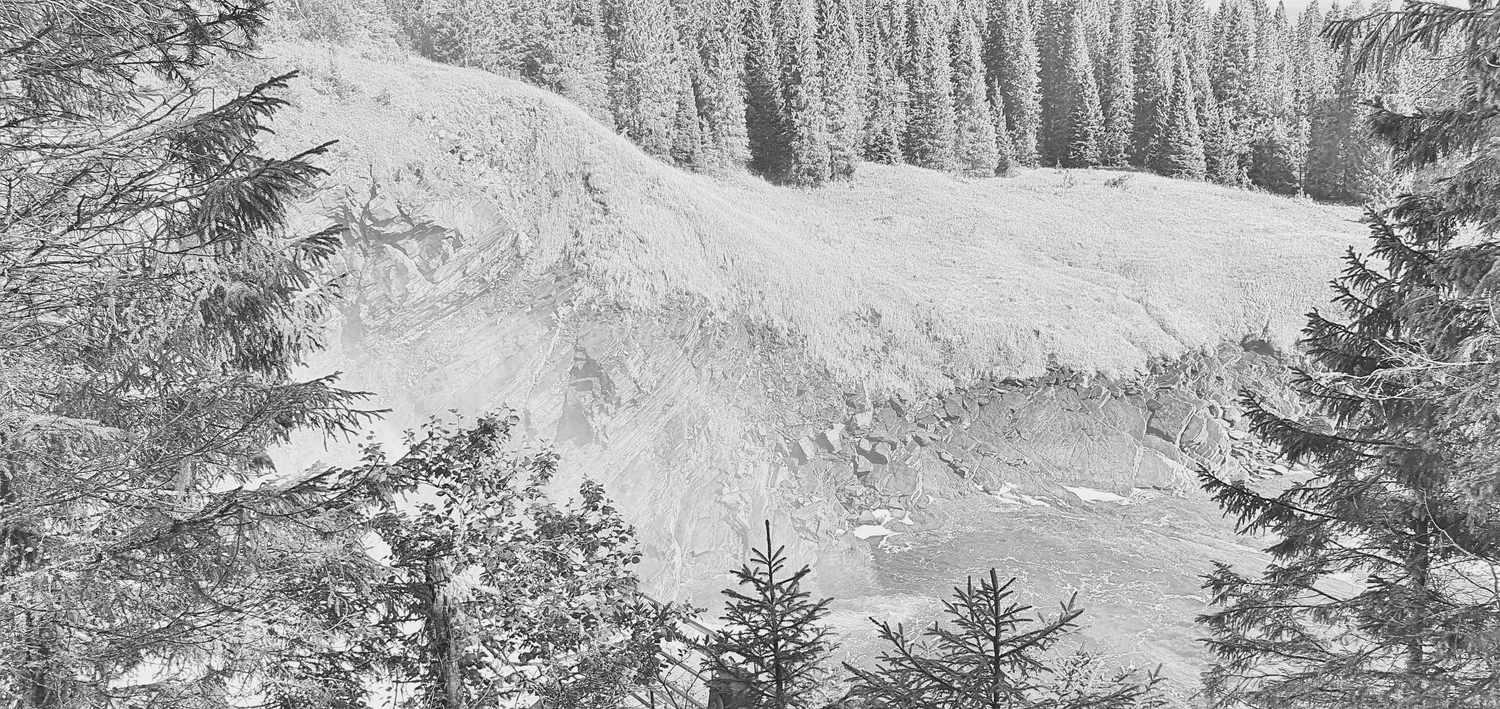
\includegraphics[width=0.50\textwidth]{plotting/examples/forsen_roundtrip.small.jpg} &
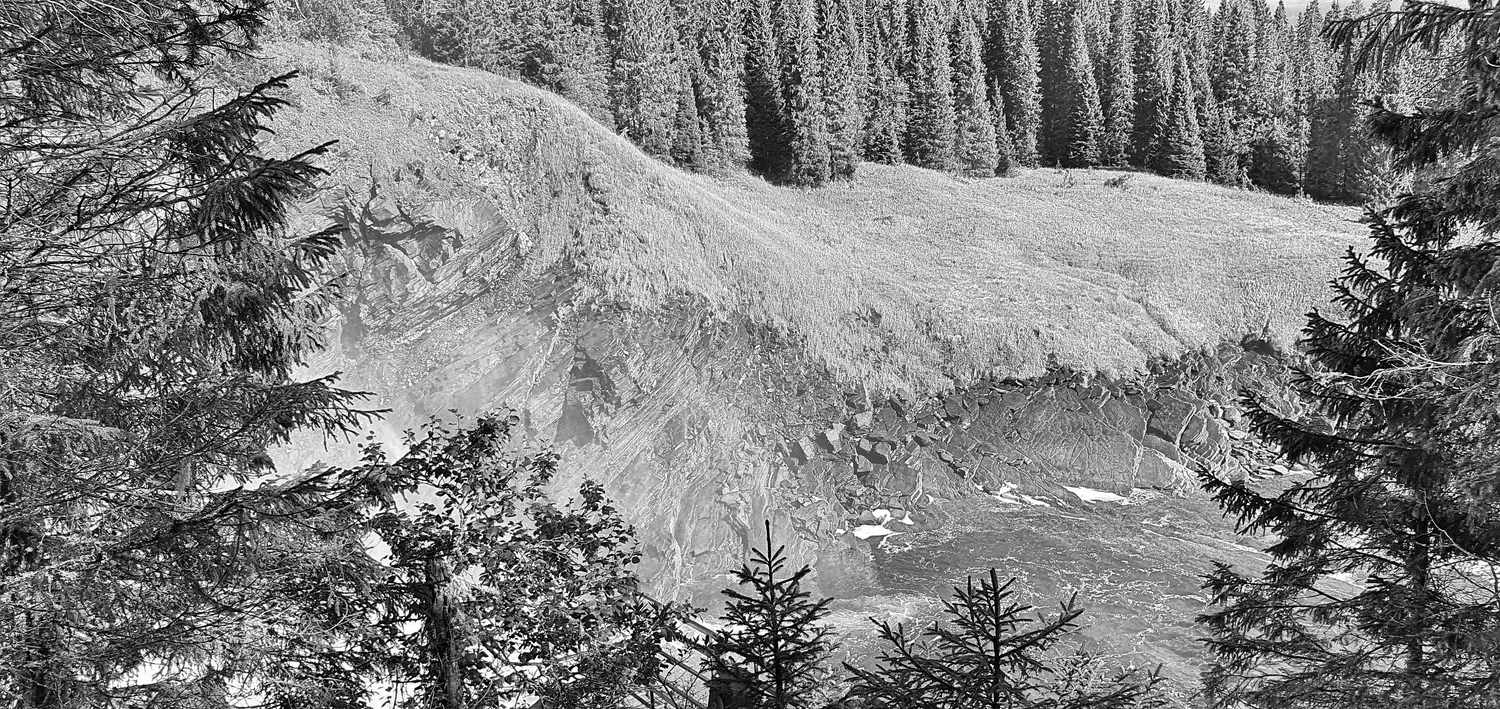
\includegraphics[width=0.50\textwidth]{plotting/examples/forsen_sort.small.jpg} \\
\hline
Equalized using multi_nth_element: m=2: & Equalized using multi_nth_element: m=5\\
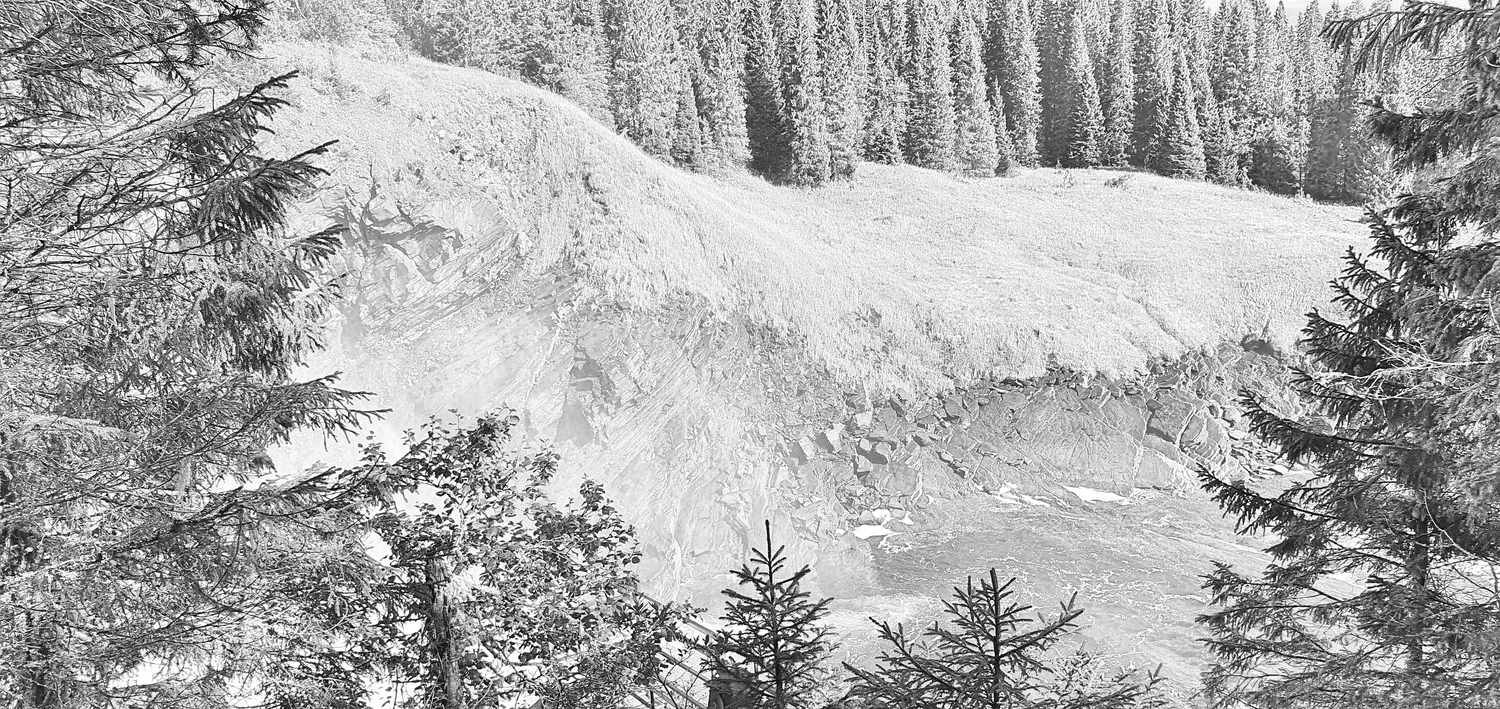
\includegraphics[width=0.50\textwidth]{plotting/examples/forsen_partition2.small.jpg} &
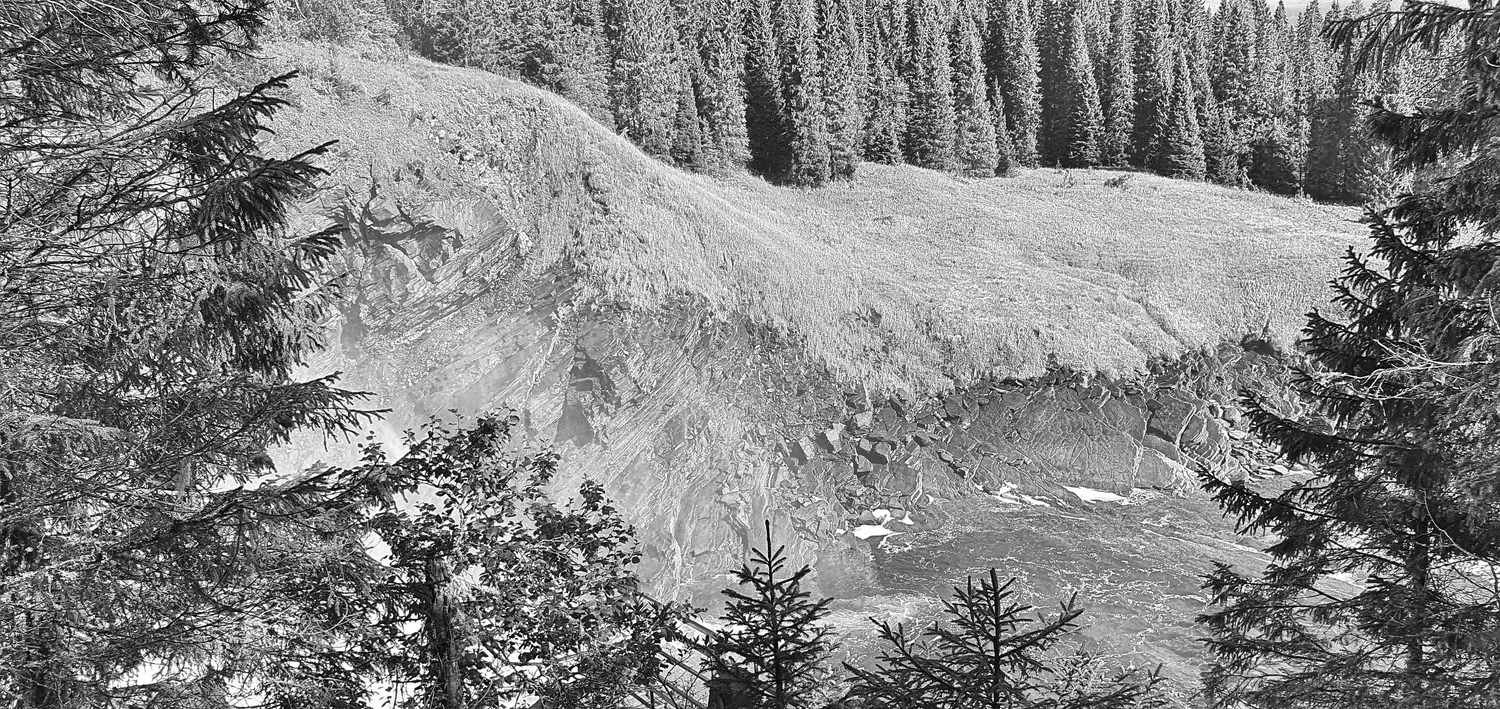
\includegraphics[width=0.50\textwidth]{plotting/examples/forsen_partition5.small.jpg}\\
\hline
\end{tabular}
\enlargethispage*{1em}

\begin{center}
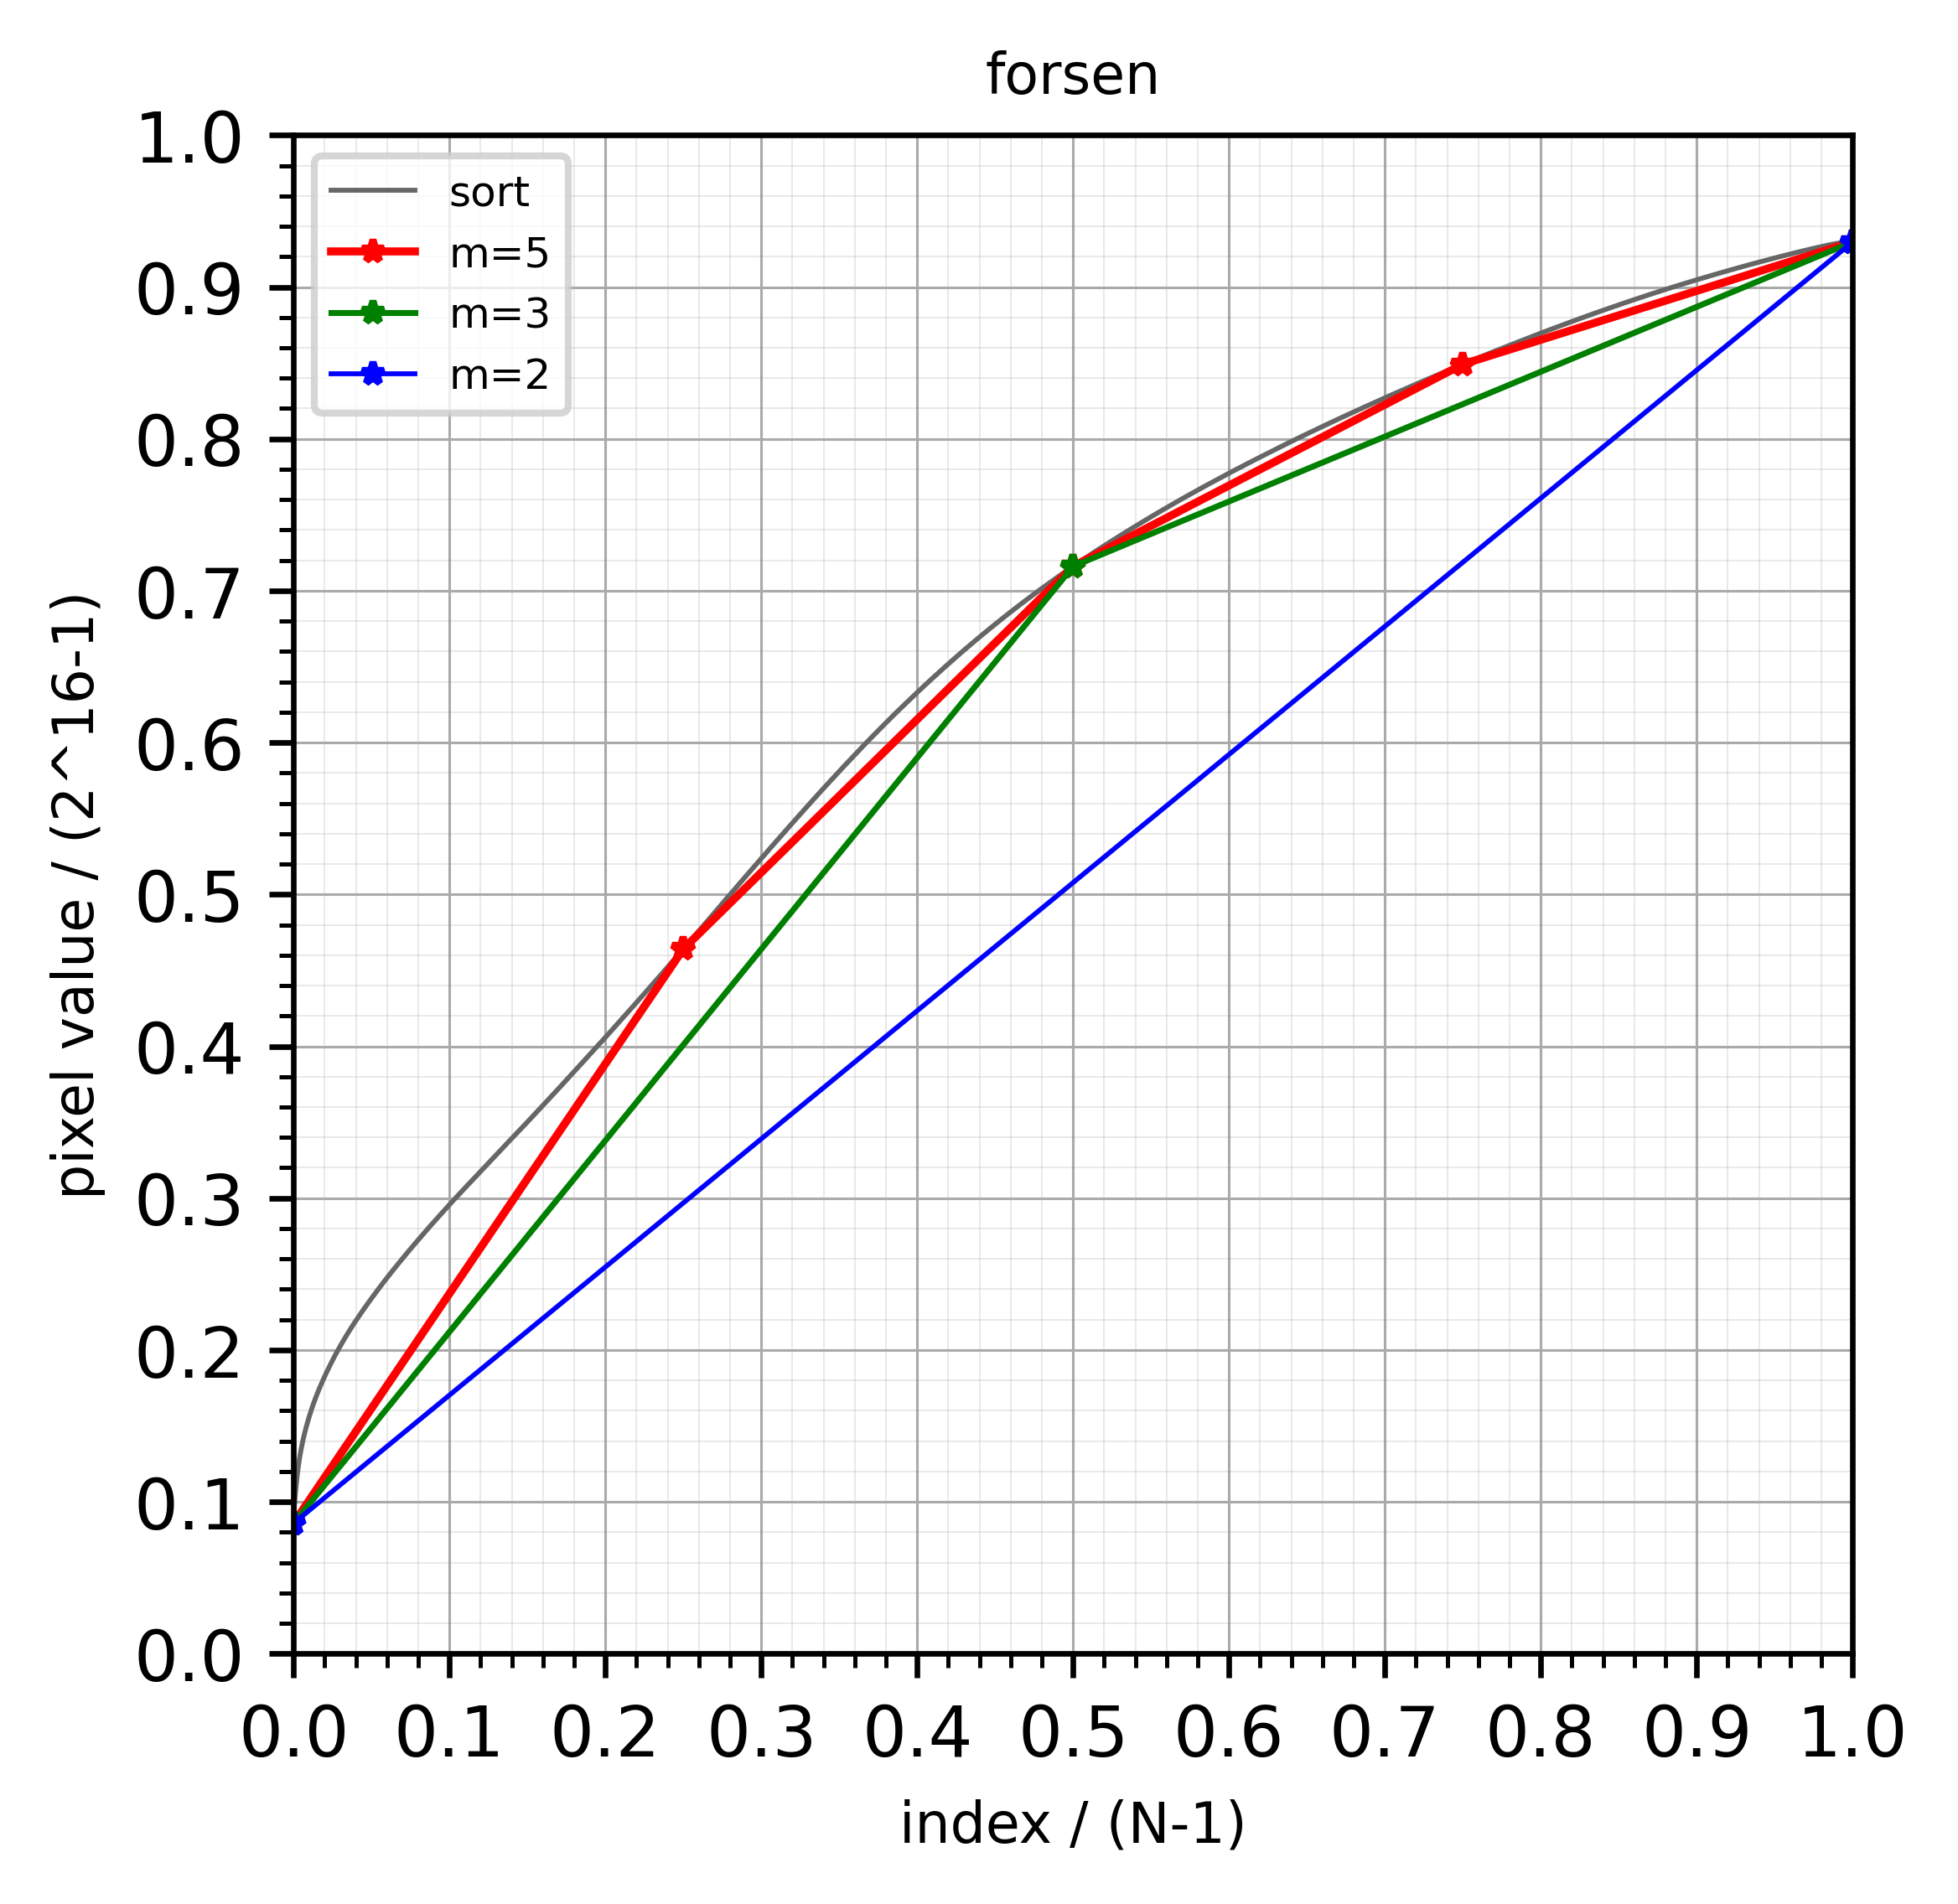
\includegraphics[width=0.55\textwidth]{plotting/examples/forsen_cdf_approximation.png}
\end{center}
Above, the exact CDF (using sort) of the original image is shown in gray, along with approximations using \emph{multi_nth_element}. At m=2, the equalization algorithm is equivalent to mapping the image min,max to grayscale values zero and 1.


\newpage
\section{Wording and Synopsis }
\label{synopsis}

\subsection{\protect{\tcode{[alg.nth.element]}}}

\added{Underlined green text} marks additions with respect to C++23 draft (2021-12-27).

\renewcommand{\tref}[1]{ ref:\emph{#1}}
\renewcommand{\iref}[1]{ ref:\emph{#1}}

\begin{itemdescr}
\pnum
Let \tcode{comp} be \tcode{less\{\}}
and \tcode{proj} be \tcode{identity\{\}}
for the overloads with no parameters by those names.

\pnum
\expects
\range{first}{nth} and \range{nth}{last} are valid ranges.
For the overloads in namespace \tcode{std},
\tcode{RandomAccessIterator} meets
the \oldconcept{ValueSwappable} requirements\iref{swappable.requirements}, and
the type of \tcode{*first} meets
the \oldconcept{MoveConstructible} (\tref{cpp17.moveconstructible}) and
\oldconcept{MoveAssignable} (\tref{cpp17.moveassignable}) requirements.
\added{For the overloads taking a range [nths_first,nths_last), RandomAccessIteratorNths is a \oldconcept{RandomAccess} iterator, and *nths_first is convertible to  RandomAccessIterator. For every iterator i and j in the range [nths_first,nths_last), it holds that if \tcodeadd{i<j} then \tcodeadd{!(*j<*i).}}

\pnum
\effects
After \tcode{nth_element} the element in the position pointed to by \tcode{nth}
is the element that would be in that position
if the whole range were sorted with respect to \tcode{comp} and \tcode{proj},
unless \tcode{nth == last}.
Also for every iterator \tcode{i} in the range \range{first}{nth}
and every iterator \tcode{j} in the range \range{nth}{last}
it holds that:
\tcode{bool(invoke(comp, invoke(proj, *j), invoke(proj, *i)))} is \tcode{false}.
\added{For the overloads taking a range of \tcodeadd{nths}, this holds for all \tcodeadd{nth} in \tcodeadd{nths}.}

\pnum
\returns
\tcode{last} for the overload in namespace \tcode{ranges}.

\pnum
\complexity
For the overloads with no \tcode{ExecutionPolicy}, linear on average.
For the overloads with an \tcode{ExecutionPolicy}, \bigoh{N} applications of
the predicate, and \bigoh{N \log N} swaps, where $N = \tcode{last - first}$.
\added{For overloads taking a range of \tcodeadd{nths} but no ExecutionPolicy, \bigoh{N~log~m} on average, where $m$ is the number of unique elements in \tcodeadd{nths}.
For overloads taking a range of \tcodeadd{nths} and an ExecutionPolicy, approximately \bigoh{N~log~N}.}
\end{itemdescr}

\subsection{Synopsis -- \tcode{<algorithm> [algorithm.syn]}}

Added signatures to \tcode{std::}

\begin{codeblockAdd}
template<class RandomAccessIterator, class RandomAccessIteratorNths>
constexpr void nth_element( RandomAccessIterator first, 
RandomAccessIteratorNths nths_first, RandomAccessIteratorNths nths_last,
RandomAccessIterator last);

template<class RandomAccessIterator, class RandomAccessIteratorNths, class Compare>
constexpr void nth_element( RandomAccessIterator first, 
RandomAccessIteratorNths nths_first, RandomAccessIteratorNths nths_last,
RandomAccessIterator last, Compare comp);
\end{codeblockAdd}
\newpage
\begin{codeblockAdd}
template<class ExecutionPolicy, class RandomAccessIterator, class RandomAccessIteratorNths>
void nth_element(ExecutionPolicy&& exec, RandomAccessIterator first, 
RandomAccessIteratorNths nths_first, RandomAccessIteratorNths nths_last,
RandomAccessIterator last);

template<class ExecutionPolicy, class RandomAccessIterator,
class RandomAccessIteratorNths, class Compare>
void nth_element(ExecutionPolicy&& exec, RandomAccessIterator first, 
RandomAccessIteratorNths nths_first, RandomAccessIteratorNths nths_last,
RandomAccessIterator last, Compare comp);

\end{codeblockAdd}

Added signatures to \tcode{std::ranges::}

\begin{codeblockAdd}
namespace ranges {
  template<@\libconcept{random_access_iterator}@ I, @\libconcept{sentinel_for}@<I> S,
  @\libconcept{random_access_range}@ Nths, class Comp = ranges::less, class Proj = identity>
  requires @\libconcept{sortable}@<I, Comp, Proj>
  && @\libconcept{convertible_to}@<iter_reference_t<iterator_t<Nths>>, I>
  constexpr I nth_element(I first, Nths&& nths, S last, Comp comp = {}, Proj proj = {});

  template<@\libconcept{random_access_range}@ R,
  @\libconcept{random_access_range}@ Nths, class Comp = ranges::less, class Proj = identity>
  requires @\libconcept{sortable}@<iterator_t<R>, Comp, Proj>
  && @\libconcept{convertible_to}@<iter_reference_t<iterator_t<Nths>>, iterator_t<R>>
  constexpr borrowed_iterator_t<R> 
  nth_element(R&& r, Nths&& nths, Comp comp = {}, Proj proj = {}); 
}

\end{codeblockAdd}
% for reference, this is the standard draft as of 2021-12-27:
%  template<@\libconcept{random_access_iterator}@ I, @\libconcept{sentinel_for}@<I> S,
%  class Comp = ranges::less, class Proj = identity>
%  requires @\libconcept{sortable}@<I, Comp, Proj>
%  constexpr I nth_element(I first, I nth, S last, Comp comp = {}, Proj proj = {});
%
%  template<@\libconcept{random_access_range}@ R, class Comp = ranges::less, class Proj = identity>
%  requires @\libconcept{sortable}@<iterator_t<R>, Comp, Proj>
%  constexpr borrowed_iterator_t<R> nth_element(R&& r, iterator_t<R> nth, Comp comp = {}, Proj proj = {});

\newpage
\section{Questions and Answers}

\subsection{Q: What's the best name?}

A: I suggest to reuse \tcode{nth_element} for discoverability but it could as well be a separate name. The name \tcode{std::nth_element} is established since pre-standard STL times ($\sim$1994?). In the literature\cite{Alsuwaiyel2001,Kaligosi2006,Panh2002,lent1996,Shen1997}, it is known as \emph{select(ion)}, and the proposed algorithm is known as \emph{multiselect(ion)}. 

As an alternative to overloading \tcode{std::nth_element}, I find it quite reasonable (and not \emph{too} creative) to follow the same pattern, with the name \tcode{std::multi_nth_element}.

Numpy overloads the name \dblquotes{\tcode{partition}} for both select and multiselect.

\subsection{Q: What about corner cases?}

Q: What if \tcode{nths} or [first,last) is empty? A: \tcode{multi_nth_element} does nothing.

Q: What if some elements of \tcode{nths} are equal to last. A: As with \tcode{nth_element}, not a problem.

Q: What if some elements of \tcode{nths} are equal to each other A: By specification, not a problem.

\subsection{Q: Is there's a need to require \tcode{nths} be \tcode{sized_range}?}

A: Not sure, I don't think so. The example implementation does not use .size().


\subsection{Q: How should the \tcode{nths} be provided?}

The current-standard single-nth version uses a single iterator \tcode{nth} to designate the location in the range. A range of iterators seems to me the most natural way to designate multiple arbitrary locations in a range.

This seem \emph{least-surprise} and offers flexibility as well as natural combination with other operations (such as seen in the examples here and in the proposal). Python uses indices rather than iterators to express locations in lists and arrays, and its incarnation of the proposed algorithm uses range-of-indices (or a single value) to specify the partition point(s)\cite{NpPart}.

\subsection{Q: Benefits and performance beyond Ordo.}

A: The comment is appreciated. Expanded the paper introduction and Examples and Application section. Added performance study, section \ref{perfstudy}.

An interesting discussion of \tcode{std::sort} vs single-nth \tcode{std::nth_element} and \tcode{std::partial_sort} is found at [CppCon 2018: Fred Tingaud "A Little Order: Delving into the STL sorting algorithms"](\url{https://www.youtube.com/watch?v=-0tO3Eni2uo})

\newpage
\section{Reference implementation and practical performance}
\label{perfstudy}

Several reference implementations and a performance study, including the code, is found at \cite{p2375RefImpl} and is summarized here.
\subsubsection*{Time vs \tcode{std::sort} for equidistant partitioning points}

\begin{center}
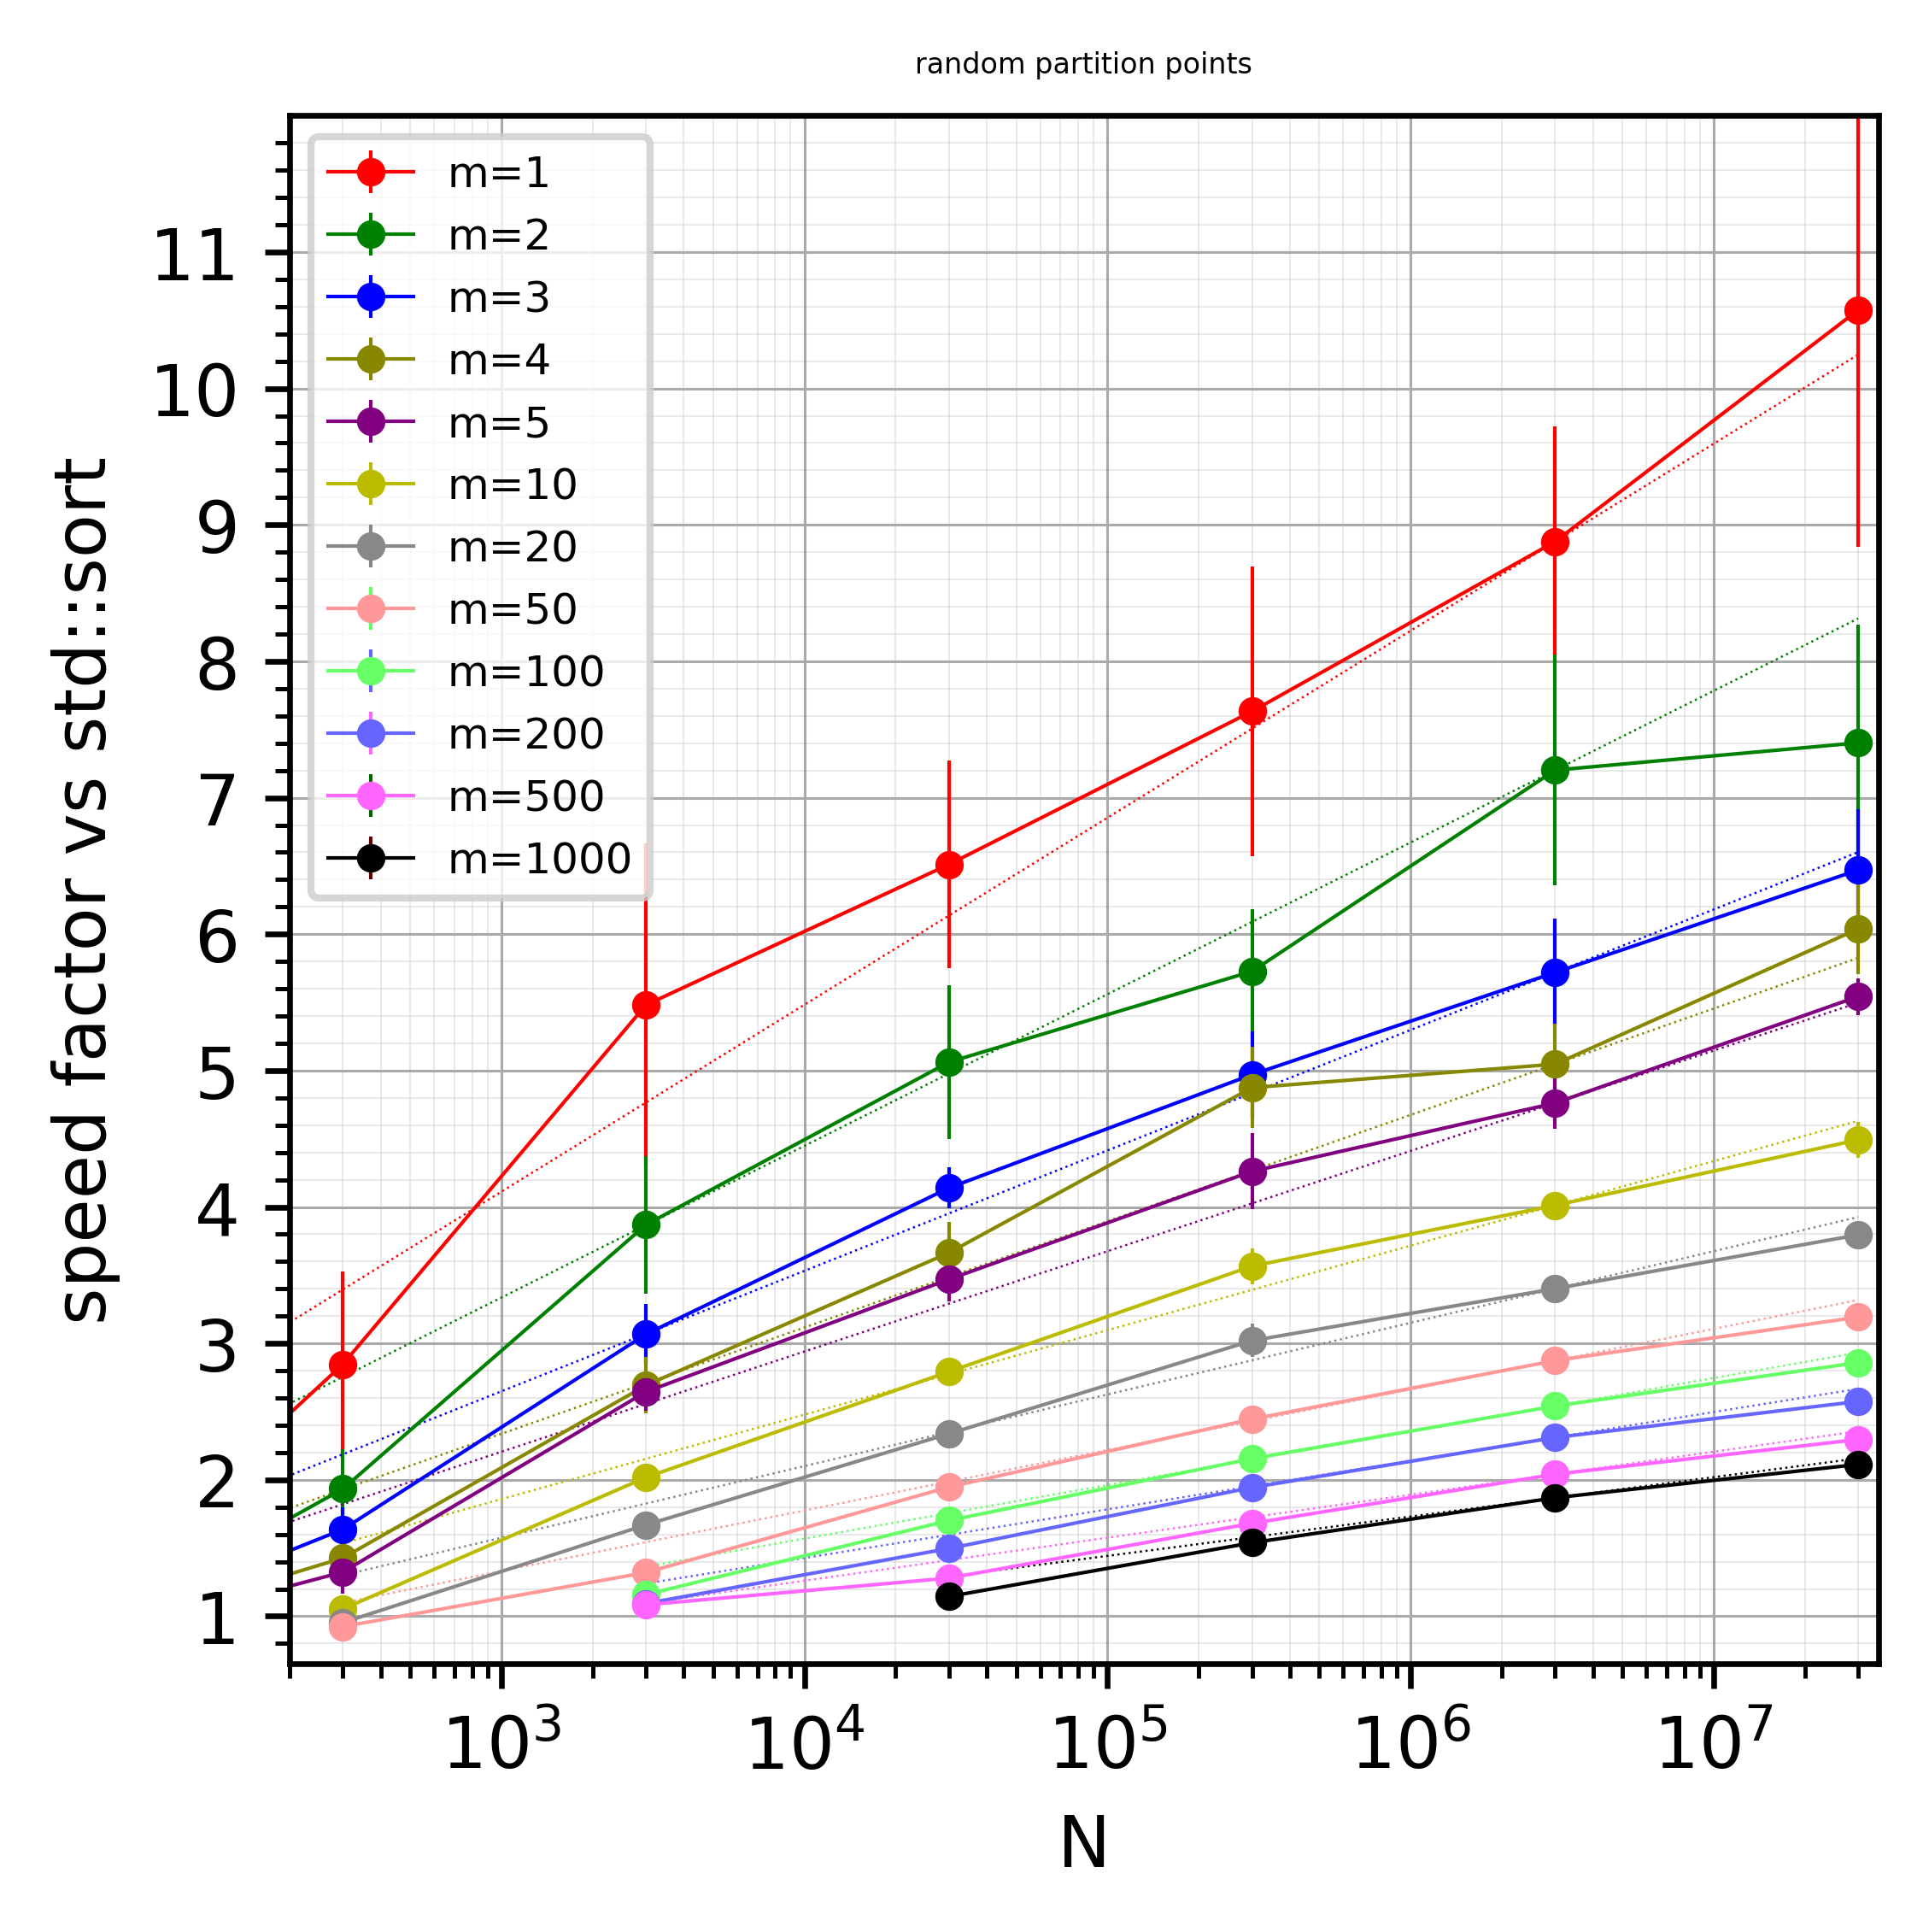
\includegraphics[width=0.55\textwidth]{plotting/images/mqs_med3_equi_speed_for_n_vs_sort.png}
\end{center}

The above image shows the execution speed of a \tcode{multi_quick_select} implementation compared to \tcode{std::sort} for various vector sizes $N$. 
Each data point is the mean of many repetitions, excluding outliers. Error bars show the spread of all repetitions and is influenced by the randomness of the test data. Individual data points do fluctuate between initial random seeds of the example, but the overall trends are very stable.

The \tcode{bisect_nths} algorithm (similar to \cite{Alsuwaiyel2001}) shown in section \ref{Implementation} is about 10\% slower for $m>5$, and about 20\% slower for $m>50$ but has the same asymptotic complexity. The data to sort here consists of randomly shuffled doubles, and \tcode{multi_nth_element} was given different numbers $m$ of evenly spaced partitioning points in the vector. Dotted lines show lines $k_i \cdot log(N)$ fitted to pass though each curve at $N=3e6$. 

The image shows that the speed curves approximately follow the expected $log(N)$ shape, with different factors for different $m$.

The following table shows a few speedup factors for a number of unique partitioning points $m$ and vector sizes $N$. 

\begin{center}
\begin{tabular}{|r|c|c|} %
  \hline 
  \textbf{m} & \textbf{speedup factor} & \textbf{at N}\\
  \hline 
1 & 10 & $N=3e7$\\
5 & 5 & $N=3e7$\\
10 & 4.5 & $N=3e7$\\
500 & 2.3 & $N=3e7$\\
1000 & 2.1 & $N=3e7$\\
\hline
10 & 3.6 & $N=3e5$\\
50 & 2.4 & $N=3e5$\\
\hline
5 & 2.6 & $N=3e3$\\
  \hline 
\end{tabular}
\end{center}

%Some care is required when interpreting the plot at low N: For example at the curve $m=1000$.
% $N=300$, the actual number of partitioning points are saturated to $N$, that is $300$ unique partitioning points. 

Clearly, the benefit compared to  \tcode{std::sort} is the greatest for smaller $m$. In these tests of  \tcode{multi_quick_select}, the performance are still not worse than \tcode{std::sort} even for $m \sim N$. 
The benefit over \tcode{sort} grows with $N$ as $log N$. Further slices and ways to plot the same performance data is found at \cite{p2375RefImpl}. It also shows the study repeated for uniformly random (unique) partition points with very similar conclusion, but slightly better performance.

\section*{Acknowledgements}
\addcontentsline{toc}{section}{Acknowledgements}

Many thanks to undisclosed proofreaders and to 
Albin Fredriksson and Marco Rubini for helpful discussions. Many thanks to all who gave comments and feedback.

\renewcommand{\bibname}{References}
\bibliographystyle{abstract}
\bibliography{ref}

\renewcommand{\addcontentsline}[3]{}% Make \addcontentsline a no-op
\begin{thebibliography}{9}
\oldaddcontentsline{toc}{section}{References}

\bibitem[StepLee95]{StepLee95}
Alexander Stepanov and Meng Lee: The Standard Template Library.\\HP Laboratories Technical Report 95-11(R.1), November 14, 1995 \\
\url{http://stepanovpapers.com/STL/DOC.PDF }

\bibitem[Alsuwaiyel2001]{Alsuwaiyel2001} 
Muhammad H. Alsuwaiyel: An optimal parallel algorithm for the multiselection problem. 
Parallel Computing Volume 27, Issue 6, May 2001, Pages 861-865\\
\url{https://doi.org/10.1016/S0167-8191(00)00095-8 }

\bibitem[Kaligosi2006]{Kaligosi2006}
Towards Optimal Multiple Selection\\ 
Kanela Kaligos,Kurt Mehlhorn, J. Ian Munro, Peter Sanders --
July 2005 Lecture Notes in Computer Science 3580:103-114 --
DOI:10.1007/11523468_9
\bibitem[Akl1984]{Akl1984} 
S. G. Akl, Optimal parallel algorithms for computing convex hulls and for sorting, Computing, 33 (1984), 1-11.
\bibitem[Akl1989]{Akl1989} 
S. G. Akl, The Design and Analysis of Parallel Algorithms (PrenticeHall, Englewood Cliffs, New Jersey, 1989).
%M. L. Fredman and T. H. Spencer, Refined complexity analysis for heap operations, Journal of Computer and
%System Sciences, (1987), 269-284.
\bibitem[Shen1997]{Shen1997} 
H. Shen, Optimal parallel multiselection on EREW PRAM, Parallel Computing, 23(1997), 1987-1992.

\bibitem[NpPart]{NpPart}
Python numpy.partition \\
\url{https://numpy.org/doc/stable/reference/generated/numpy.partition.html }

\bibitem[NPImpl]{NPImpl}
The implementation of partition (multiple and single nth version) is found at
{\footnotesize \url{https://github.com/numpy/numpy/blob/v1.20.2/numpy/core/src/multiarray/item_selection.c#L1023 }}

\bibitem[Musser1997]{Musser1997}
David R. Musser, Introspective Sorting and Selection Algorithms\\
Software--Practice and Experience, (8): 983-993 (1997))\\
\url{https://www.cs.rpi.edu/~musser/gp/algorithms.html }

\bibitem[Panh2002]{Panh2002}
Alois Panholzer --
Analysis of multiple quickselect variants\\
Theoretical Computer Science
Volume 302, Issues 1–3, 13 June 2003, Pages 45-91\\
\url{https://doi.org/10.1016/S0304-3975(02)00729-6 }

\bibitem[lent1996]{lent1996}
Janice Lent, Hosam M.Mahmoud\\
Average-case analysis of multiple Quickselect: An algorithm for finding order statistics\\
Statistics \& Probability Letters \\
Volume 28, Issue 4, August 1996, Pages 299-310
\url{https://doi.org/10.1016/0167-7152(95)00139-5}


\bibitem[p2375RefImpl]{p2375RefImpl}
 Reference Implementation, Performance study and usage examples on \emph{this} proposal.\\
\url{https://github.com/jmlundberg/nth_element_material}

\bibitem[p2375src]{p2375src}
Document source and status page for \emph{this} proposal.\\
\url{https://github.com/jmlundberg/p2375}

\end{thebibliography}
\let\addcontentsline\oldaddcontentsline% Restore \addcontentsline

\end{document}
